\subsubsection{MLL-AF4 and RUNX1 cooperate to regulate apoptosis, and may promote Venetoclax insensitivity}

While MLL-FPs are well known prevent apoptosis through \textit{BCL2} overexpression \citep{benito_mll-rearranged_2015}, additional apoptosis components may be important. The BCL2 inhibitor venetoclax is a successful treatment for \textit{MLL}r leukaemias \citep{khaw_venetoclax_2016, vandenberg_abt-199_2013}, yet there is variable response with in vitro models \citep{pan_selective_2014} and drug resistance is a concern. MLL-FP circuits may elucidate alternative mechanisms \textit{MLL}r leukaemias may prevent apoptosis and escape venetoclax treatment. To identify candidate nodes that confer resistance to venetoclax I used a CRISPR screen combined with drug treatment, performed by Max Jamilly (\cite{harman_kmt2a-aff1_2021}, see methods, \ref{fig:ch4_max}A-B). This screen was performed in THP-1 cells (MLL-AF9 AML), and while this differs from SEM (MLL-AF4 ALL) lineage switching is known to occur between ALL and AML leukaemias under selective pressure \citep{gardner_acquisition_2016, pillai_car_2019} and core regulatory logic is similar (See Fig. \ref{fig:ch4_sem-thp1}). Unfortunately due to poor reproducibility with DMSO treatment, rather than comparing T18 DMSO with T18 venetoclax, we compared T0 baseline with T18 venetoclax. As such, significant hits require additional validation (Fig. \ref{fig:ch4_max}C). 

\begin{figure}[h]
    \centering
    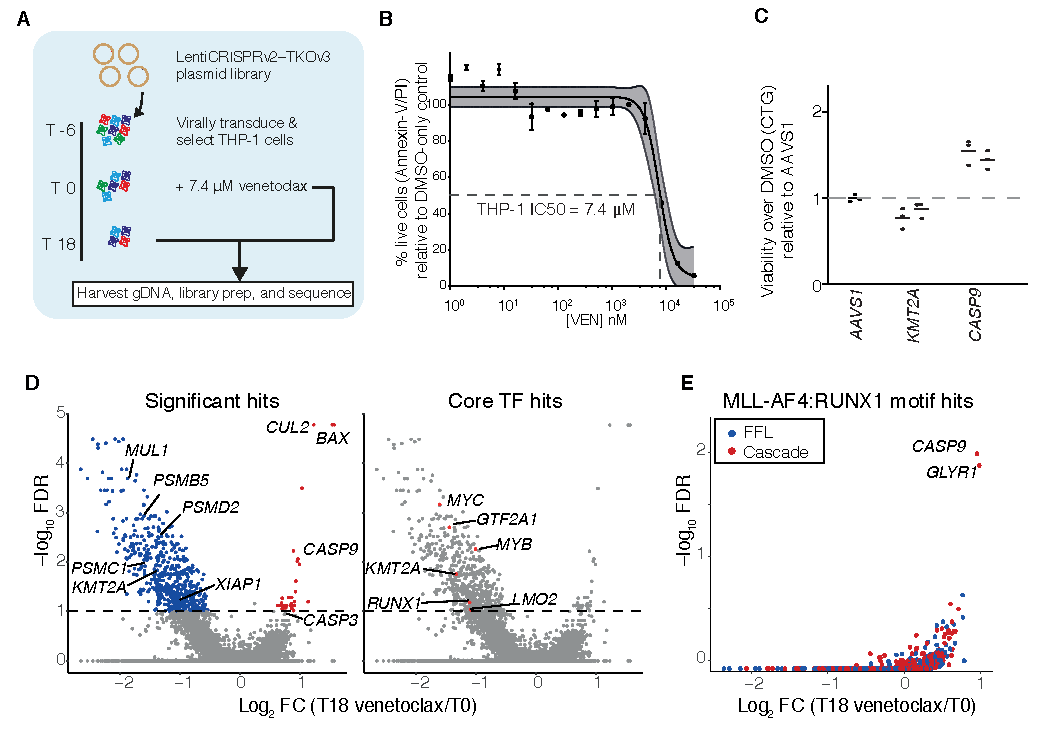
\includegraphics[width=\textwidth,height=\textheight,keepaspectratio]{figures/chapter4/ch4_max.png}
    %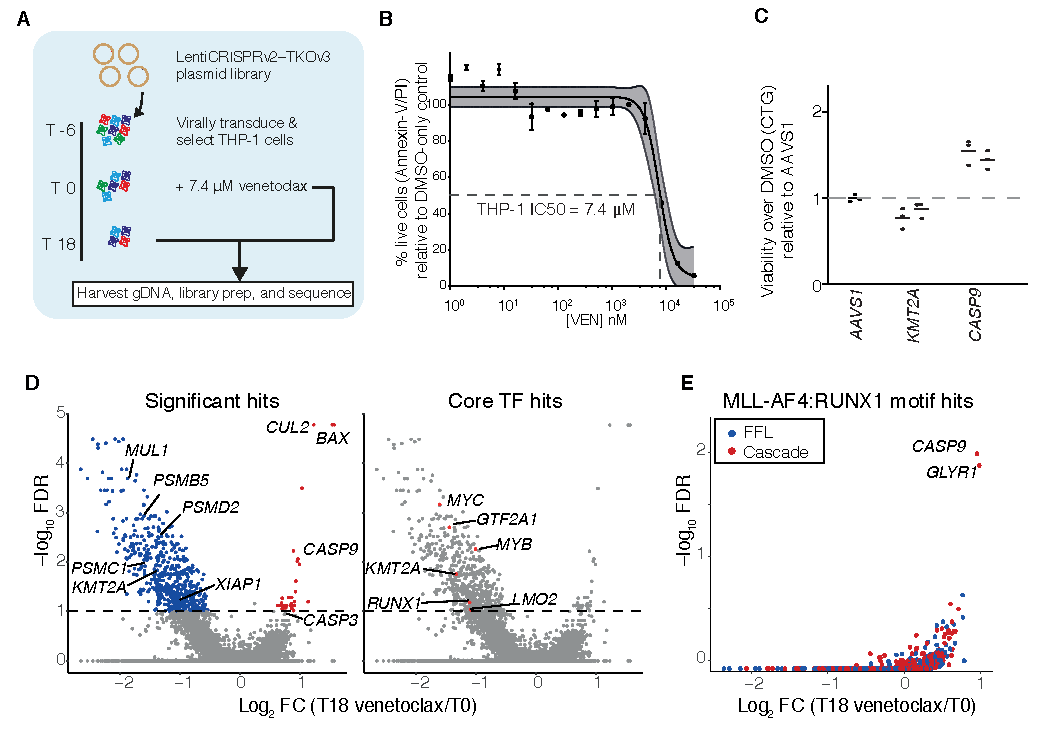
\includegraphics{figures/chapter4/ch4_max.png}
    \caption[{Venetoclax screen.}]
    {\textbf{Venetoclax screen.} 
    \textbf{(A)} Illustration outlining CRISPR screen conducted in combination with 7.4 \microm{} (IC50) venetoclax treatment in THP-1 cells. See methods for details. 
    \textbf{(B)} THP-1 IC50 estimation with 48 hour' venetoclax treatment in THP-1 cells. Viability assayed with Annexin-V/PI staining. Data points show mean; error bars show SD. Lines show unconstrained four parameter sigmoidal least-squares regression with 99\% CI. (\textit{n} = 5). 
    \textbf{(C)} Validation of CRISPR screen hits with 48 hours' DMSO or 20 \microm{} venetoclax treatment in CRISPR edited THP-1 cells. sgRNAs used were from the Brunello library. CTG was used to assay viability, normalised as venetoclax/DMSO relative to \textit{AAVS1} silent control. Bars indicate mean. (\textit{n} = 3). 
    \textbf{(D)} MAGeCK analysis of CRISPR screen comparing T0 (baseline) and T18 (venetoclax), plotting -log\textsubscript{10} FDR against log\textsubscript{2} sgRNA FC. (Left) Key significant genes within the GRN; (right) core GRN TFs. 
    \textbf{(E)} Enriched genes as in D, showing MLL-AF4:RUNX1 FFL and cascade targets. 
    \textit{CRISPR screen and validations performed by Max Jamilly (A-C). GRN integration with MAGeCK analysis performed by myself. Adapted from \cite{harman_kmt2a-aff1_2021}.}
    }
    \label{fig:ch4_max}
\end{figure}

Among MLL-AF4 GRN regulated genes, several sgRNA targeting central nodes were depleted (perturbation inhibits survival) after venetoclax treatment, including \textit{RUNX1} and \textit{MLL} (\textit{MLL-AF9}) (Fig. \ref{fig:ch4_max}D). This suggests these core TFs generally promote cell growth and survival. Genes perturbations that promote venetoclax resistance will have enriched sgRNA after drug treatment. \textit{CASP9} (caspase-9) is the most significantly enriched hit that is also a target of a MLL-AF4:RUNX1 motif, and has been independently validated (Fig. \ref{fig:ch4_max}C, E). Perturbation of caspase-9 confers survival, consistent with its role in apoptosis \citep{li_caspases_2008, li_cytochrome_1997, slee_ordering_1999}. 

\textit{CASP9} is partially repressed in a TF cascade where 96 hours' \textit{MLL-AF4} or \textit{RUNX1} KD increased expression (Fig. \ref{fig:ch4_casp9}A-B). Stable KO of \textit{CASP9} in SEM cells reproduced venetoclax resistance (Fig. \ref{fig:ch4_casp9}C-D, Appendix \ref{fig:app_casp9-del}). These KO lines displayed variable RUNX1 protein and mRNA levels though this did not correlate with \textit{CASP9} status, and is likely a result of clonal expansion (Fig. \ref{fig:ch4_casp9}C). \textit{MLL-AF4} KDs were performed for 96 hours for robust loss of protein, however this favours secondary effects. A reduced \textit{MLL-AF4} KD for 48 hours does not reduce overall RUNX1 protein, and has little effect on \textit{CASP9} expression (P = 0.64, Fig. \ref{fig:ch4_casp9}F-G). With 48 hours' \textit{RUNX1} KD \textit{CASP9} is upregulated, in both SEM and RS4;11 cells (Fig. \ref{fig:ch4_casp9}F, H-I). Together these results evidence a true MLL-AF4:RUNX1:\textit{CASP9} TF cascade, where repression is directly driven by RUNX1. Further, repression of \textit{CASP9} may reduce sensitivity to venetoclax.

\begin{figure}[ht]
    \centering
    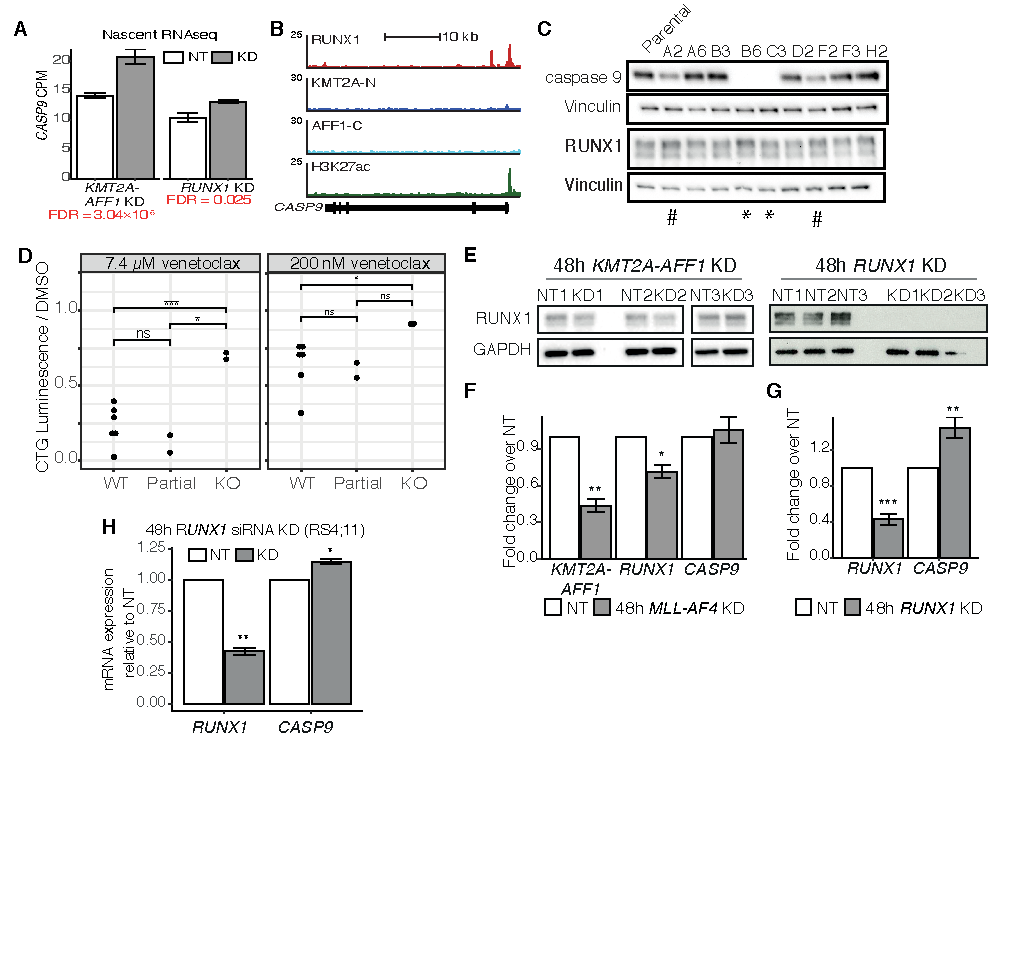
\includegraphics[width=0.8\textwidth,height=0.8\textheight,keepaspectratio]{figures/chapter4/ch4_casp9.png}
    %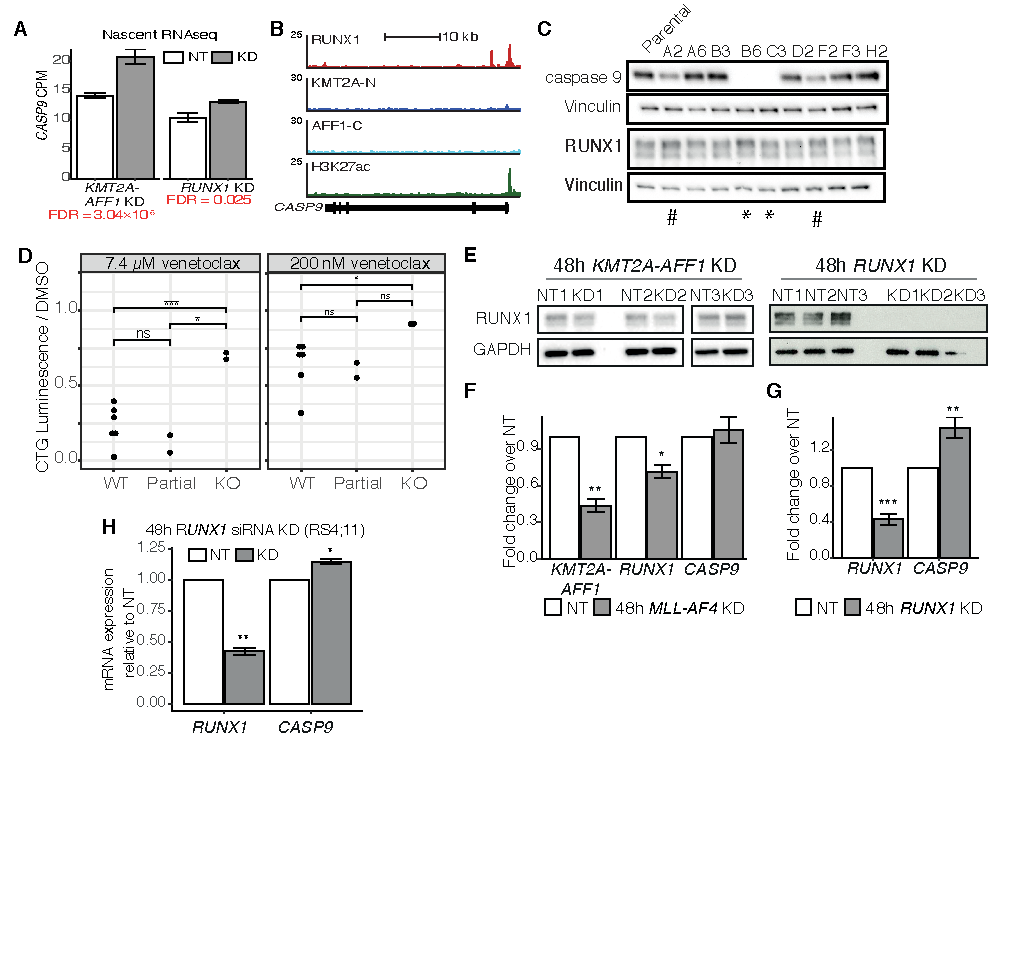
\includegraphics{figures/chapter4/ch4_casp9.png}
    \caption[{Casp9.}]
    {\textbf{Casp9.} 
    \textbf{(A)} \textit{CASP9} expression following 96 hours’ \textit{MLL-AF4} KD, normalized as CPM. 
    \textbf{(B)} ChIP-seq tracks at the \textit{CASP9} locus. 
    \textbf{(C)} Western blot for caspase-9 and RUNX1 in \textit{CASP9} knockout SEM clones. Vinculin used as loading control. Full and partial KO indicated with a * and \#, respectively. Parental refers to original, unedited cell line. 
    \textbf{(D)} CTG viability assay in \textit{CASP9} KO clones following 48 hours’ treatment with 7.4 \microm{} venetoclax (left) or 200 nM venetoclax (IC50 in SEM cells, as in \cite{benito_mll-rearranged_2015}) (right). CTG luminescence displayed relative to DMSO control. Individual clones used as biological replicates (WT \textit{n} = 5, KO and partial KO \textit{n} = 2). 
    \textbf{(E)} Western blot for RUNX1 protein in SEM cells after 48 h \textit{MLL-AF4} KD or 48 h \textit{RUNX1} KD, with GAPDH as loading control. 
    \textbf{(F, G, H)} qRT-PCR assaying \textit{MLL-AF4}, \textit{RUNX1} and \textit{CASP9} expression following 48 h \textit{MLL-AF4} KD (F) or 48 h \textit{RUNX1} KD (G) in SEM cells or RS4;11 cells (H) (\textit{n} = 3). Expression normalized to GAPDH and shown relative to NT control. 
    \textit{Adapted from \cite{harman_kmt2a-aff1_2021}.}
    }
    \label{fig:ch4_casp9}
\end{figure}

This analysis presents RUNX1 as a novel target to enhance venetoclax efficacy. In fact, recent studies have noted improved venetoclax response in patients with RUNX1 mutations \citep{cherry_venetoclax_2021, chow_runx1_2021}. Treating SEM cells with a small molecule RUNX1 inhibitor (active AI-10-104, inactive AI-4-88) that disrupts RUNX1 binding to CBF$\beta$ \citep{illendula_small-molecule_2015, illendula_small_2016} resulted in partially reduced RUNX1 DNA binding and expression (Fig. \ref{fig:ch4_runx1-inh}A-B). Dose-response curves were generated using variable venetoclax concentrations and 10 \microm{} RUNX1 inhibitor. Co-treatment with AI-10-104 yielded lower venetoclax IC50 (78nM) over AI-4-88 or DMSO treatment (208.97nM, 193.47nM) (Fig. \ref{fig:ch4_runx1-inh}C). This preliminary analysis suggests an interaction between venetoclax and RUNX1 activity, though \textit{CASP9} levels appear unaffected by RUNX1 inhibitors (Fig. \ref{fig:ch4_runx1-inh}B). It has been proposed that RUNX1 perturbation improves venetoclax response through generally reducing the apoptotic threshold \citep{chow_runx1_2021}. A more robust experimental design is required to determine if the effect is synergistic.

\begin{figure}[ht]
    \centering
    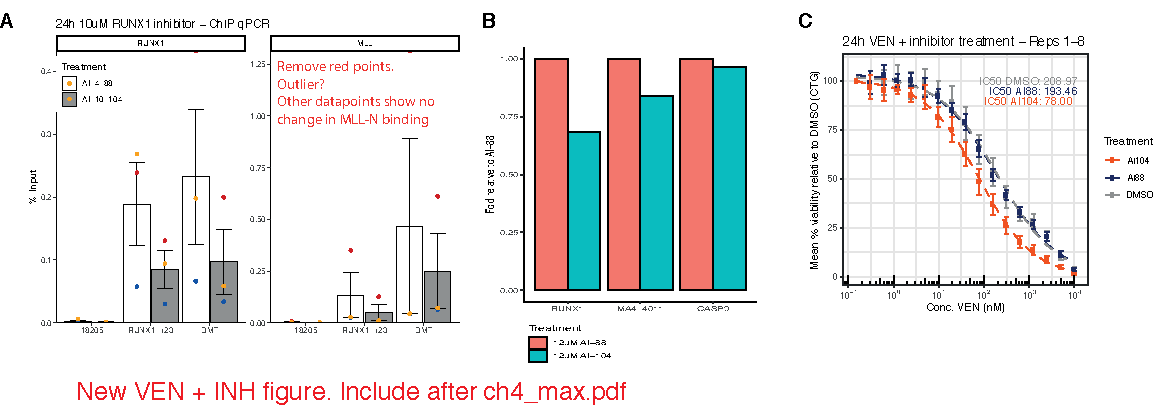
\includegraphics[width=\textwidth,height=\textheight,keepaspectratio]{figures/chapter4/chr4_runx1-inh.png}
    %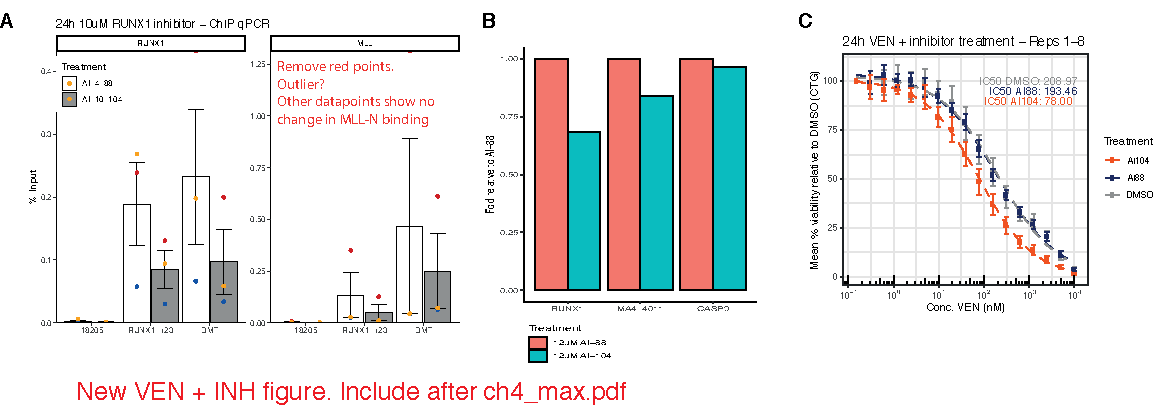
\includegraphics{figures/chapter4/chr4_runx1-inh.png}
    \caption[{Runx1 inhibitor x venetoclax.}]
    {\textbf{Runx1 inhibitor x venetoclax.} 
    \textbf{(A)} RUNX1 and MLL-N ChIP qPCR after 24 h 10 \microm{} AI-10-104 or AI-4-88 (as used in SEM cells in \cite{illendula_small_2016}), normalised to input chromatin. Regions probed are the \textit{RUNX1} +23 enhancer and a RUNX1 bound peak at the \textit{BMF} locus. Bars show mean, and error bars represent SE (\textit{n} = 3).
    \textbf{(B)} qRT-PCR analysis showing \textit{RUNX1}, \textit{MLL-AF4}, and \textit{CASP9} expression after 24 h 10 \microm{} AI-10-104 or AI-4-88 treatment (\textit{n} = 1). Expression normalised to GAPDH shown relative to AI-4-88.
    \textbf{(C)} Dose response curve of venetoclax concentrations treated in SEM cells for 24 h. Cells were co-treated with 10 \microm{} AI-10-104, AI-4-88 or DMSO). Viability measured using CTG, normalised to DMSO control. Dashed line represents dose response curve fit, and IC50 was calculated in the context of RUNX1 inhibitors. (\textit{n} = 8). 
    }
    \label{fig:ch4_runx1-inh}
\end{figure}